\documentclass[tikz,border=9pt]{standalone}
\usepackage{fontspec}
\setmainfont{TeX Gyre Heros}
\usepackage{amsmath}
\usepackage{unicode-math}
\setmathfont{TeX Gyre Termes Math}
\usepackage{pgfplots}
\usepgfplotslibrary{fillbetween,groupplots}
\usetikzlibrary{arrows.meta,calc}
\definecolor{maroon}{HTML}{780404}
\definecolor{orange}{HTML}{E37D00}
\definecolor{charcoal}{HTML}{303238}
\definecolor{muted}{HTML}{65686D}
\definecolor{gridgray}{HTML}{DDDFE2}
\pgfplotsset{compat=1.18,
  oscillator/.style={
    width=12.6cm,height=8.8cm,
    xmin=-3.5,xmax=3.5,ymin=0,ymax=5.35,
    axis lines=left,axis line style={charcoal,line width=.7pt,-{Stealth[length=4pt]}},
    xtick={-3,-2,-1,0,1,2,3},ytick={0,1,2,3,4,5},
    tick align=outside,tick style={charcoal},
    tick label style={font=\small,text=charcoal},
    xlabel={$q=x/\ell$},ylabel={$\varepsilon=E/(\hbar\omega)$},
    label style={font=\normalsize,text=charcoal},
    xlabel style={at={(axis description cs:.5,-.085)},anchor=north},
    ylabel style={at={(axis description cs:-.075,.5)},anchor=south},
    ymajorgrids=true,grid style={gridgray,dashed,line width=.35pt},
    clip=false,samples=251,
  },
}
\begin{document}
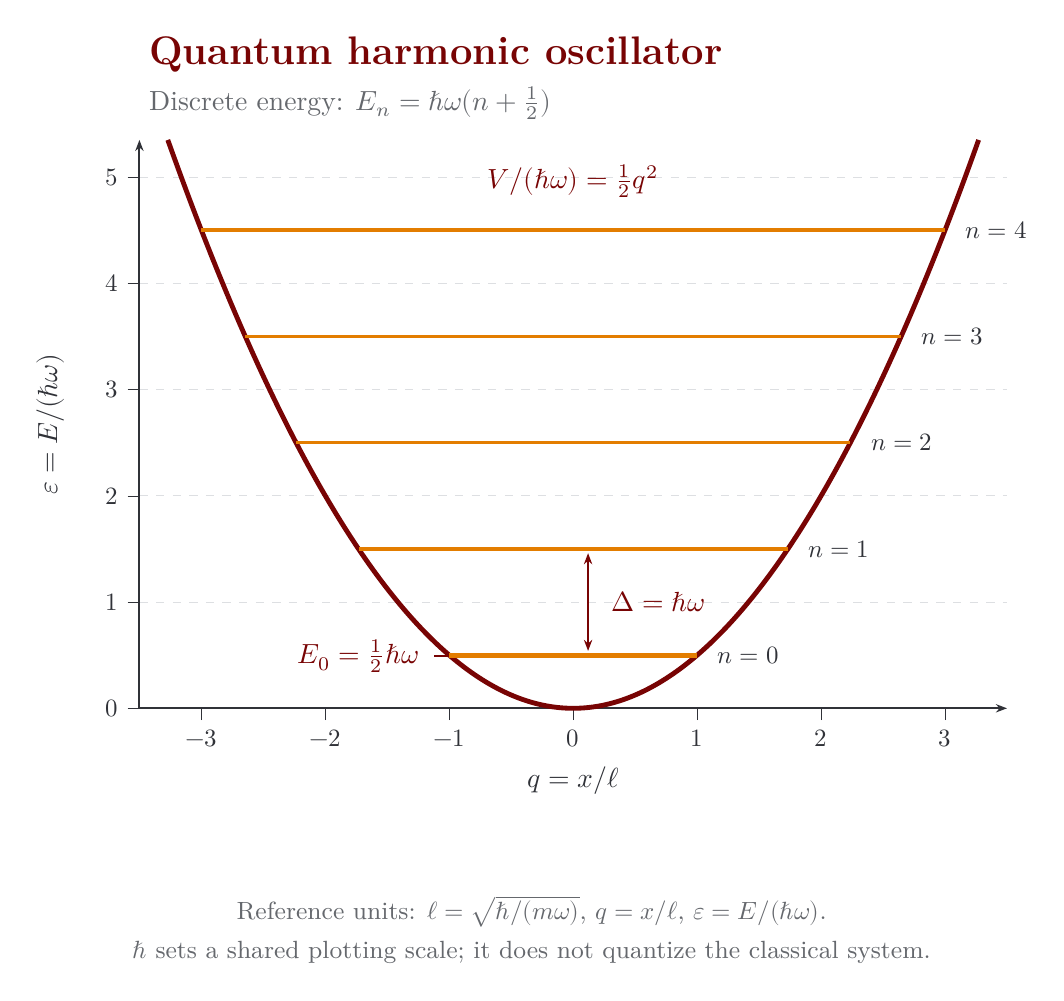
\begin{tikzpicture}[text=charcoal]
\begin{axis}[oscillator]

\node[anchor=west,font=\Large\bfseries,text=maroon]
  at (axis description cs:0,1.15) {Quantum harmonic oscillator};
\node[anchor=west,font=\normalsize,text=muted]
  at (axis description cs:0,1.065) {Discrete energy: $E_n=\hbar\omega(n+\tfrac12)$};

\addplot[maroon,line width=1.75pt,domain=-3.271085:3.271085] {.5*x^2};
\node[font=\normalsize,text=maroon,anchor=north]
  at (axis cs:0,5.21) {$V/(\hbar\omega)=\tfrac12q^2$};

\addplot[orange,line width=1.8pt] coordinates {(-1.0000000000,0.5) (1.0000000000,0.5)};
\node[anchor=west,font=\small,text=charcoal,xshift=4pt]
  at (axis cs:1.0000000000,0.5) {$n=0$};

\addplot[orange,line width=1.25pt] coordinates {(-1.7320508076,1.5) (1.7320508076,1.5)};
\node[anchor=west,font=\small,text=charcoal,xshift=4pt]
  at (axis cs:1.7320508076,1.5) {$n=1$};

\addplot[orange,line width=1.25pt] coordinates {(-2.2360679775,2.5) (2.2360679775,2.5)};
\node[anchor=west,font=\small,text=charcoal,xshift=4pt]
  at (axis cs:2.2360679775,2.5) {$n=2$};

\addplot[orange,line width=1.25pt] coordinates {(-2.6457513111,3.5) (2.6457513111,3.5)};
\node[anchor=west,font=\small,text=charcoal,xshift=4pt]
  at (axis cs:2.6457513111,3.5) {$n=3$};

\addplot[orange,line width=1.25pt] coordinates {(-3.0000000000,4.5) (3.0000000000,4.5)};
\node[anchor=west,font=\small,text=charcoal,xshift=4pt]
  at (axis cs:3.0000000000,4.5) {$n=4$};

\draw[maroon,line width=.9pt,{Stealth[length=4pt]}-{Stealth[length=4pt]}]
  (axis cs:.12,.54) -- (axis cs:.12,1.46);
\node[anchor=west,font=\normalsize,text=maroon,xshift=5pt]
  at (axis cs:.12,1) {$\Delta=\hbar\omega$};
\node[anchor=east,font=\normalsize,text=maroon]
  at (axis cs:-1.17,.49) {$E_0=\tfrac12\hbar\omega$};
\draw[maroon,line width=.55pt] (axis cs:-1.12,.49)--(axis cs:-1.01,.49);
\end{axis}

\node[anchor=north,align=center,text=muted,font=\small,yshift=-30pt]
  at (current bounding box.south) {Reference units: $\ell=\sqrt{\hbar/(m\omega)}$, $q=x/\ell$, $\varepsilon=E/(\hbar\omega)$.\\[3pt]
  $\hbar$ sets a shared plotting scale; it does not quantize the classical system.};
\end{tikzpicture}
\end{document}
